\documentclass{article}
\usepackage[margin=0.2in,paperwidth=9in,paperheight=5.2in]{geometry}
\pagestyle{empty}
\usepackage{amsmath,amssymb}
\usepackage{tikz}
\usetikzlibrary{shapes.geometric, arrows.meta, positioning, calc}

\begin{document}
\noindent
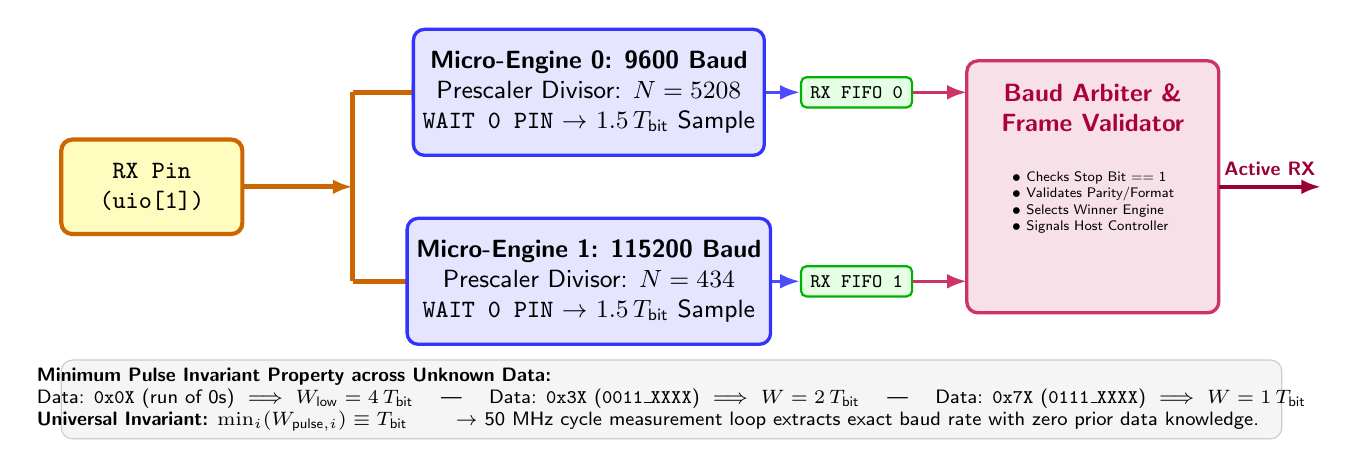
\begin{tikzpicture}[
    engine/.style={draw=blue!80, fill=blue!10, line width=1.2pt, rounded corners=4pt, minimum width=3.8cm, minimum height=1.6cm, align=center, font=\small\sffamily},
    fifo/.style={draw=green!70!black, fill=green!10, thick, rounded corners=2pt, font=\scriptsize\ttfamily},
    sig/.style={line width=1.2pt, -{Latex[length=2.5mm]}},
    txt/.style={font=\scriptsize\sffamily}
]

% Input Physical Pin
\draw[fill=yellow!25, draw=orange!80!black, line width=1.5pt, rounded corners=4pt] (-0.5, 2.0) rectangle (1.8, 3.2);
\node[font=\small\bfseries\ttfamily, align=center] at (0.65, 2.6) {RX Pin\\(uio[1])};

% Fanout Wire
\draw[sig, line width=1.8pt, orange!80!black] (1.8, 2.6) -- (3.2, 2.6);
\draw[line width=1.8pt, orange!80!black] (3.2, 3.8) -- (3.2, 1.4);
\draw[sig, line width=1.8pt, orange!80!black] (3.2, 3.8) -- (4.2, 3.8);
\draw[sig, line width=1.8pt, orange!80!black] (3.2, 1.4) -- (4.2, 1.4);

% Micro-Engine 0 (9600 Baud)
\node[engine] (e0) at (6.2, 3.8) {
    \textbf{Micro-Engine 0: 9600 Baud} \\
    Prescaler Divisor: $N = 5208$ \\
    \texttt{WAIT 0 PIN} $\rightarrow$ $1.5\,T_{\text{bit}}$ Sample
};

% Micro-Engine 1 (115200 Baud)
\node[engine] (e1) at (6.2, 1.4) {
    \textbf{Micro-Engine 1: 115200 Baud} \\
    Prescaler Divisor: $N = 434$ \\
    \texttt{WAIT 0 PIN} $\rightarrow$ $1.5\,T_{\text{bit}}$ Sample
};

% FIFOs
\node[fifo] (f0) at (9.6, 3.8) {RX FIFO 0};
\node[fifo] (f1) at (9.6, 1.4) {RX FIFO 1};
\draw[sig, blue!70] (e0.east) -- (f0.west);
\draw[sig, blue!70] (e1.east) -- (f1.west);

% Arbiter / Selection Logic
\draw[fill=purple!12, draw=purple!80, line width=1.2pt, rounded corners=4pt] (11.0, 1.0) rectangle (14.2, 4.2);
\node[font=\small\bfseries\sffamily, text=purple!90!black, align=center] at (12.6, 3.6) {Baud Arbiter \&\\Frame Validator};
\node[font=\tiny\sffamily, align=left] at (12.6, 2.4) {
    $\bullet$ Checks Stop Bit == 1 \\
    $\bullet$ Validates Parity/Format \\
    $\bullet$ Selects Winner Engine \\
    $\bullet$ Signals Host Controller
};
\draw[sig, purple!80] (f0.east) -- (11.0, 3.8);
\draw[sig, purple!80] (f1.east) -- (11.0, 1.4);

% Output to Host
\draw[sig, line width=1.5pt, purple!80!black] (14.2, 2.6) -- (15.5, 2.6) node[midway, above, font=\scriptsize\bfseries\sffamily] {Active RX};

% Bottom Comparison Box: Unknown Data Pulses
\draw[fill=gray!8, draw=gray!40, rounded corners=4pt] (-0.5, -0.6) rectangle (15.0, 0.4);
\node[font=\scriptsize\sffamily, align=left] at (7.25, -0.1) {
    \textbf{Minimum Pulse Invariant Property across Unknown Data:} \\
    Data: \texttt{0x0X} (run of 0s) $\implies W_{\text{low}} = 4\,T_{\text{bit}}$ \quad | \quad
    Data: \texttt{0x3X} (\texttt{0011\_XXXX}) $\implies W = 2\,T_{\text{bit}}$ \quad | \quad
    Data: \texttt{0x7X} (\texttt{0111\_XXXX}) $\implies W = 1\,T_{\text{bit}}$ \\
    \textbf{Universal Invariant:} $\min_{i} (W_{\text{pulse}, i}) \equiv T_{\text{bit}}$ \qquad
    $\rightarrow$ 50 MHz cycle measurement loop extracts exact baud rate with zero prior data knowledge.
};

\end{tikzpicture}
\end{document}
